\documentclass[12pt]{book}
\usepackage[width=4.375in, height=7.0in, top=1.0in, papersize={5.5in,8.5in}]{geometry}
%\usepackage[pdftex]{graphicx}
\usepackage{amsmath}
\usepackage{amssymb}
\usepackage{tipa}
%for using the euro sign
\usepackage{eurosym}
\usepackage{graphicx}
%\usepackage{txfonts}
\usepackage{textcomp}
%\usepackage{amsthm}
%\usepackage{array}
%\usepackage{xy}
\usepackage{fancyhdr}

\pagestyle{fancy}
\renewcommand{\chaptermark}[1]{\markboth{#1}{}}
\renewcommand{\sectionmark}[1]{\markright{\thesection\ #1}}
\fancyhf{}
\fancyhead[LE,RO]{\bfseries\thepage}
\fancyhead[LO]{\bfseries\rightmark}
\fancyhead[RE]{\bfseries\leftmark}
\renewcommand{\headrulewidth}{0.5pt}
\renewcommand{\footrulewidth}{0pt}
\addtolength{\headheight}{0.5pt}
\setlength{\footskip}{0in}
\renewcommand{\footruleskip}{0pt}
\fancypagestyle{plain}{%
\fancyhead{}
\renewcommand{\headrulewidth}{0pt}
}
%
%\parindent 0in
\parskip 0.05in
%
\begin{document}
\frontmatter
\pagestyle{empty}
%\pagenumbering{}
% Set book title
\title{\textbf{A course on Wireless Sensor Networks (WSNs)}}
% Include Author name and Copyright holder name
\author{Luis Sanabria, Jaume Barcelo}
% 1st page for the Title
%-------------------------------------------------------------------------------
\maketitle
%
\tableofcontents
%
\mainmatter
%
\chapter{About the course}

\section{Course Data}

Code: 21754

Course name: ``Xarxes de Sensors Sense Fils''

Teacher: Luis Sanabria and Jaume Barcelo

Credits: 4

Year: 3rd or 4th year (optional)

Trimester: Spring

\section{Introduction}
The reduction in price and size of computing and wireless communication platforms over the last years opens a new possibility for gathering and processing information: Wireless Sensor Networks.
A wireless sensor node is an electronic device of small dimensions that gathers measures from the environment and transmit the data wirelessly.
In wireless sensor nodes, communication is often established with other wireless sensor nodes to exchange or pass information.
It is common to have this data directed to an special device that gathers all the data and is called the network sink.
As wireless sensor nodes are often battery-powered, energy saving is a relevant issue in these networks.

What follows is an extract of the first pages of \cite{sanabria2012lpw}.

\begin{quotation}
Wireless Sensor Networks (WSNs) are a result of significant breakthroughs on wireless transceiver technology, the need of event sensing and monitoring. One might think of a WSN as the skin of our bodies; apart from its importance on many other subjects, our skin senses events nearby it, like touch, temperature changes, pressure and so forth. These events are generated by an external entity, the nerves or sensors of our skin are capable to react to such events and transmit this information to the brain. \\

There are enormous differences among characteristics of WSN and the skin, but the example given above will work as head start to understanding the technology. For instance, our skin sends the sensed event information towards the brain through the nerves, we could safely relate this medium to a wired network infrastructure. While in WSN, as its name suggests sends the sensed data towards a central node (Sink) via a wireless medium. Because of the limited radio range of each node, the route to the Sink is generally composed of jumps through different nodes (which is called a multi-hop route).\\

The majority of wireless nodes in a WSN are very constrained devices due to the restrictions in costs and sometimes harsh environments where these networks are deployed. These constraints go from cost, processing power, memory, storage, radio range, spectrum and, more importantly, battery life. One of the most popular low-end nodes model, the TelosB, is equipped with $16$ MHz CPU, very small flash memory ($48$ KB avg.), about $10$ KB of RAM and works on the very crowded $2.4$ GHz spectrum at rates around $250$ Kbps. These limitations force WSN engineers to design applications capable of working with low processor-intensive tasks and powered with limited battery (usually two AA batteries).\\

Many WSN applications process the sensed event before sending the data, this processing tries to reduce the information to send. As mentioned in \cite{akyildiz2010wireless}, it is less energy consuming to process one bit of information than sending it. WSN protocols and applications are tailored to power conservation rather than throughput, mainly due to cost, dimension, processing and power constraints.\\

WSNs may contain different kind of sensors that help monitor metrics related to: temperature, humidity, pressure, speed, direction, movement, light, soil makeup, noise levels, presence or absence of certain kinds of objects, mechanical stress and vibration. Also further information like node location can be derived from a Global Positioning System (GPS) device embedded at each node.\\

Because of the variety of measures than can be monitored with these small and (generally) cheap devices, a wide range of applications have been developed; the authors of \cite{akyildiz2010wireless} divide them in: military, environmental, health, home and industry applications.\\

\begin{itemize}
    \item \emph{Military Applications:} one of the first applications of WSNs. The main advantages in this area are the fact that the deployment of low cost sensors (that are subject to destruction in a battlefield) proposes a cheaper approach to sensing different types of metrics, which in turn brings new challenges to WSN applications (increased power and processing constraints). Some of the applications are related to: monitoring the movement of troops, equipment and ammunition, battlefield surveillance, terrain reconnaissance, damage assessments, snipper detection \cite{ledeczi2005countersniper}, \cite{mazurek2005boomerang} and threat detection, as in the case of biological, radiological or chemical attacks.\\
    \item \emph{Environmental Applications:} most of these applications are related to animal tracking, weather conditions and threat contention \cite{polastre2004analysis}, \cite{szewczyk2004habitat}.\\
    \item \emph{Health Applications:} a great deal of these applications are dedicated to monitor patients inside hospitals and provide them with better care. This is achieved by tracking the patientÕs vitals or other information of interest and making it available to doctors at any time from anywhere securely through the Internet. \\
    \item \emph{Home Applications:} technology is making its way inside our homes from various fronts, and WSN are no exception. Sensor nodes inside domestic devices will result in an increased interaction among them and allow access via the Internet. Theses applications are of great importance in fields like domotics towards a smart home/work environment. Home surveillance and multimedia WSNs for home environments are also a growing field of research.\\
    \item \emph{Industrial Applications:} historically the monitoring of material fatigue was made by experts introducing the observed situation inside PDA devices to be collected on a central site for processing. Further sensing techniques were developed on the form of wired sensors; nevertheless its implementation was slow and expensive due the necessary wiring. WSNs bring the best of both methods by sensing the events without the need of expert personnel and the cost of wiring. \\
    \item Other implementations as mentioned in \cite{akyildiz2010wireless} are: inventory management, product quality monitoring, smart offices/houses; guidance in automatic manufacturing environments, interactive museums, factory process control and automation, machine diagnosis, transportation, vehicle tracking and detection, spectrum sensing for cognitive radio networks, underground and underwater monitoring. \\
\end{itemize}

\end{quotation}

\section{Syllabus}
\begin{itemize}
  \item Lectures
  \begin{enumerate}
    \item Introduction to WSNs.
    \item Arduino Platform.
    \item XBee and XBee explorer. AT commands.
    \item XBee API mode.
    \item A sensor network with Arduino.
    \item A sensor network without Arduino.
    \item Publishing sensed data
    \item Invited talk
    \item Quiz
  \end{enumerate}
  \item Labs and seminars
  \begin{enumerate}
    \item Blinking LED (Dimming optional)
    \item Blinking LED with push-button (dimming optional)
    \item XBee chat
    \item Wireless doorbell
    \item Sunset sensor
    \item Sensor network with Arduino
    \item Sensor network with XBee in API mode
    \item Sleeping and actuating
    \item Uploading sensed data to the Internet
  \end{enumerate}
\end{itemize}

\section{Bibliography}

Most of the lab assignments follow the book that you can find at the university library:

Robert Faludi ``Building Wireless Sensor Networks'' (\cite{faludi2010bws}).

The following list of ``common mistakes'' can be very useful when debugging your projects:

\url{http://www.faludi.com/projects/common-xbee-mistakes/}

Check also:

Massimo Banzi ``Getting Started with Arduino''.

\section{Evaluation Criteria}

The grading is distributed as follows:
\begin{itemize}
\item Quiz, 10\%
\item Each lab assignment, 10\%
\end{itemize}

It is necessary to obtain a decent mark in all the different evaluation aspects.
To pass the course, 50 out of the total 100 points need to be obtained.

\section{Team work}

You will work in teams of three people.
Try to make the groups as heterogeneous as possible: people that are experienced with Arduino and people that are not, people from different majors, people with strong programming skills and people good at electronics, etc.

Each group delivers a single report per session and the teachers may ask questions to individual members of the team.

\section{Use your imagination}
The lab assignments are somewhat easy.
The goal is that you complement what you do in the lab with other ideas of your own.
You are encouraged to explore WSNs beyond the basics introduced in the assignments and document your findings in the reports.
Doing something on your own beyond the assignment takes a lot of effort and is time-consuming.
Nevertheless, as engineers, we should be able to come up with new ideas and solutions on our own.

\section{Non-stop Arduino}
In our school there are two additional courses that make use Arduino: ``Sensors and data acquisition'' and ``Interactive Systems''.

\section{Survival guide}

\subsection{Questions and doubts}
We like to receive questions and comments.
Normally, the best moment to express a doubt is during the class, as it is likely that many people in the class share the same doubt.
If you feel that you have a question that needs to be discussed privately, we can discuss it right after the class.

\subsection{Continuous feedback}
At the end of the lecture, we will ask you to anonymously provide some feedback on the course \emph{\color{blue}{\href{http://bit.ly/10tXjX4}{using a form like this one}}}.
In particular, I always want to know:
\begin{itemize}
\item What is the most interesting thing we have seen in class.
\item What is the most confusing thing in the class.
\item Any other comment you may want to add.

In labs, I will ask each group to hand in a short (few paragraphs) description of the work carried out in class, and the members of the group that have attended the class.
Note that this is different from the deliverables, which are the ones that are actually graded.
\end{itemize}

\subsection{How to make you teachers happy}

Avoid speaking while we are talking.

\chapter{Introduction to Arduino}

\section{Open Hardware}
\emph{"There's a fine line between open source and stupidity"}, says Massimo Banzi to a reporter from Wired Magazine while having dinner at a restaurant in Milan. 

Banzi is the man behind Arduino, an open hardware platform. The open about it relates to the fact that the device's manufacturing schematics, programming language and software development environment are free and open source. This basically means that everyone interested on building hardware-coupled solutions may take an Arduino board's schematics, modify it at will, send the new design to a China manufacturer and get the final product back home for around \EUR{10}~\cite{wiredOpenHardware}.

Open hardware is supported by a variety of available licenses (like open software with LGPL, GPL, Copyleft, and others) that ensure that the protected platform can be copied, enhanced and even sold, but always recognizing the original authors. It also ensures that the resulting products are open as the original.

\section{The Arduino Platform}
Arduino was developed to teach Interaction Design~\cite{banzi2008getting}, that meant that it required the ability to sense the surroundings and do something about it.

The platform is equipped with simple digital and analog input/output interfaces, that can be programmed to sense or react to some events. Figure~\ref{fig:ArduinoBoard} shows the Arduino Duemilanove board.

\begin{figure}[htbp]
  \centering
  \includegraphics[width=0.7\linewidth]{figures/duemilanove.eps}
  \caption{Arduino Duemilanove board
  \label{fig:ArduinoBoard}}
\end{figure}

There are numerous sensors and actuators that work with Arduino. In relation to sensors: temperature, air pollution, light, GPS modules and sound are among the popular; as LEDs, speakers and digital/analog outputs are common actuators. Also, interfaces like buttons can be programmed and used as a human interactive input.

The design and electrical components of the Arduino board are available for anyone~\cite{Arduino}. Figure~\ref{fig:Arduino_schematics} shows the connections layout of the Duemilanove model (see Figure~\ref{fig:ArduinoBoard}).

\begin{figure}[htbp]
  \centering
  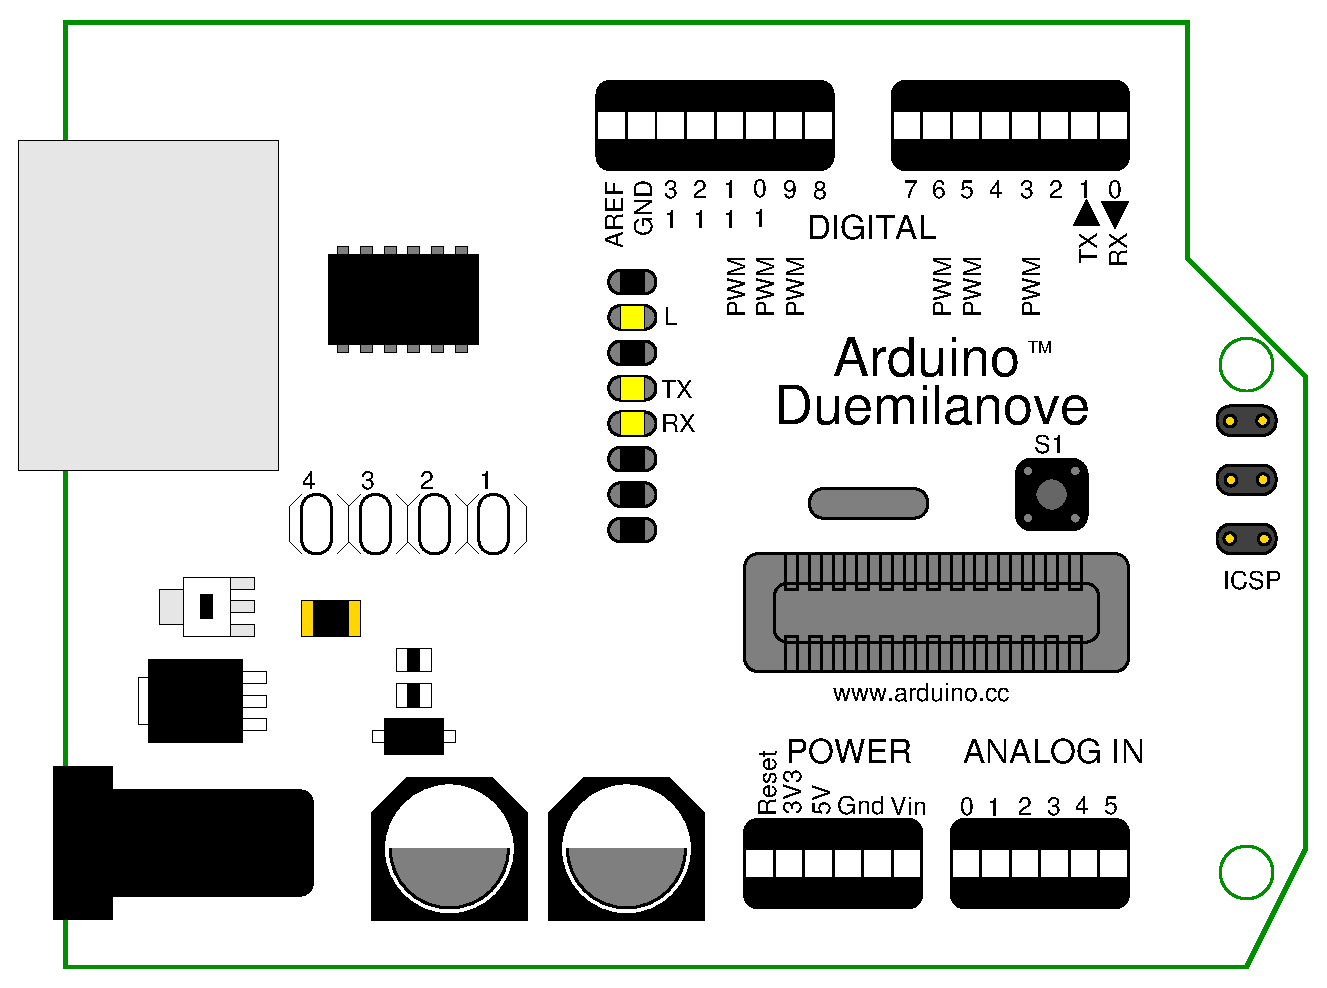
\includegraphics[width=0.7\linewidth]{figures/duemilanove_layout.eps}
  \caption{Arduino Duemilanove board: layout
  \label{fig:Arduino_schematics}}
\end{figure}

% \subsection{Developing for Arduino}

% \subsection{Example of a simple Arduino application}
\backmatter
%
\bibliographystyle{plain}
\bibliography{my_bib}
\end{document}
